\newpage
\part{Platforma Gisquick}
\newpage

\section{Úvod do Gisquick}

Gisquick je webová mapová publikační platforma s otevřenými daty. Jejím účelem je snadné a rychlé publikování projektů vytvořených v programu QGIS, které je možné posléze prohlížet webovém rozhraní platformy Quisqick. 
Celá platforma se skládá z několika komponentů (jejich obecné fungování je popsáno v Části I, kapitole 1.2). Komponenty jsou následující.

\subsection{Komponenty}

\begin{itemize}
	\item\textit{Gisquick plugin} - jedná se o zásuvný modul pro program QGIS, pomocí kterého je možné existující projekt publikovat. Použití pluginu je prvním krokem k publikaci předem vytvořeného projektu. Při publikaci si může každý uživatel pomocí pluginu projekt nastavit tak, aby zobrazovaný předmět zájmu přesně odpovídal jeho požadavkům (možnost selekce jednotlivých vrstev, nastavení maximálního a minimálního měřítka, atd.). Gisquick plugin pracuje zcela odděleně od ostatních komponentů a jeho výstupem je složka obsahující všechny použité vrstvy, uložený projekt ve formátu .qgs a metadatový soubor obsahující dodatečné nastavení projektu.
	\item\textit{webový server} - webový server zpracovává dotazy ve formě OGC standardů, které posílá klient a následně odpovídá například ve formě mapových obrazů. Na straně webového serveru je použit framework Django, který je stejně jako Gisquick plugin psaný v jazyce Python.
	\item\textit{QGIS server} - jedná se o webový mapový server na základě kterého jsou vytvářeny mapové obrazy. Použití QGIS serveru je dáno skutečností, že veškeré mapové prvky zde vytvořené korespondují svým vzhledem s těmi vytvořenými v QGIS desktopové aplikaci. Díky tomu si může být uživatel jistý tím, že to co publikuje bude věrně odpovídat jeho původnímu projektu.
	\item\textit{webový a mobilní klient} - klient uživateli nabízí uživatelské rozhraní celé aplikace ve kterém se může orientovat a pomocí kterého interaguje s webovým serverem a tak mění zobrazovaný obsah. Právě této části spolu s Gisquick Pluginem byla je v této práci věnována největší pozornost.
\end{itemize}

\subsection{Uživatelské rozhraní}

\begin{figure}[h!]
	\centering
	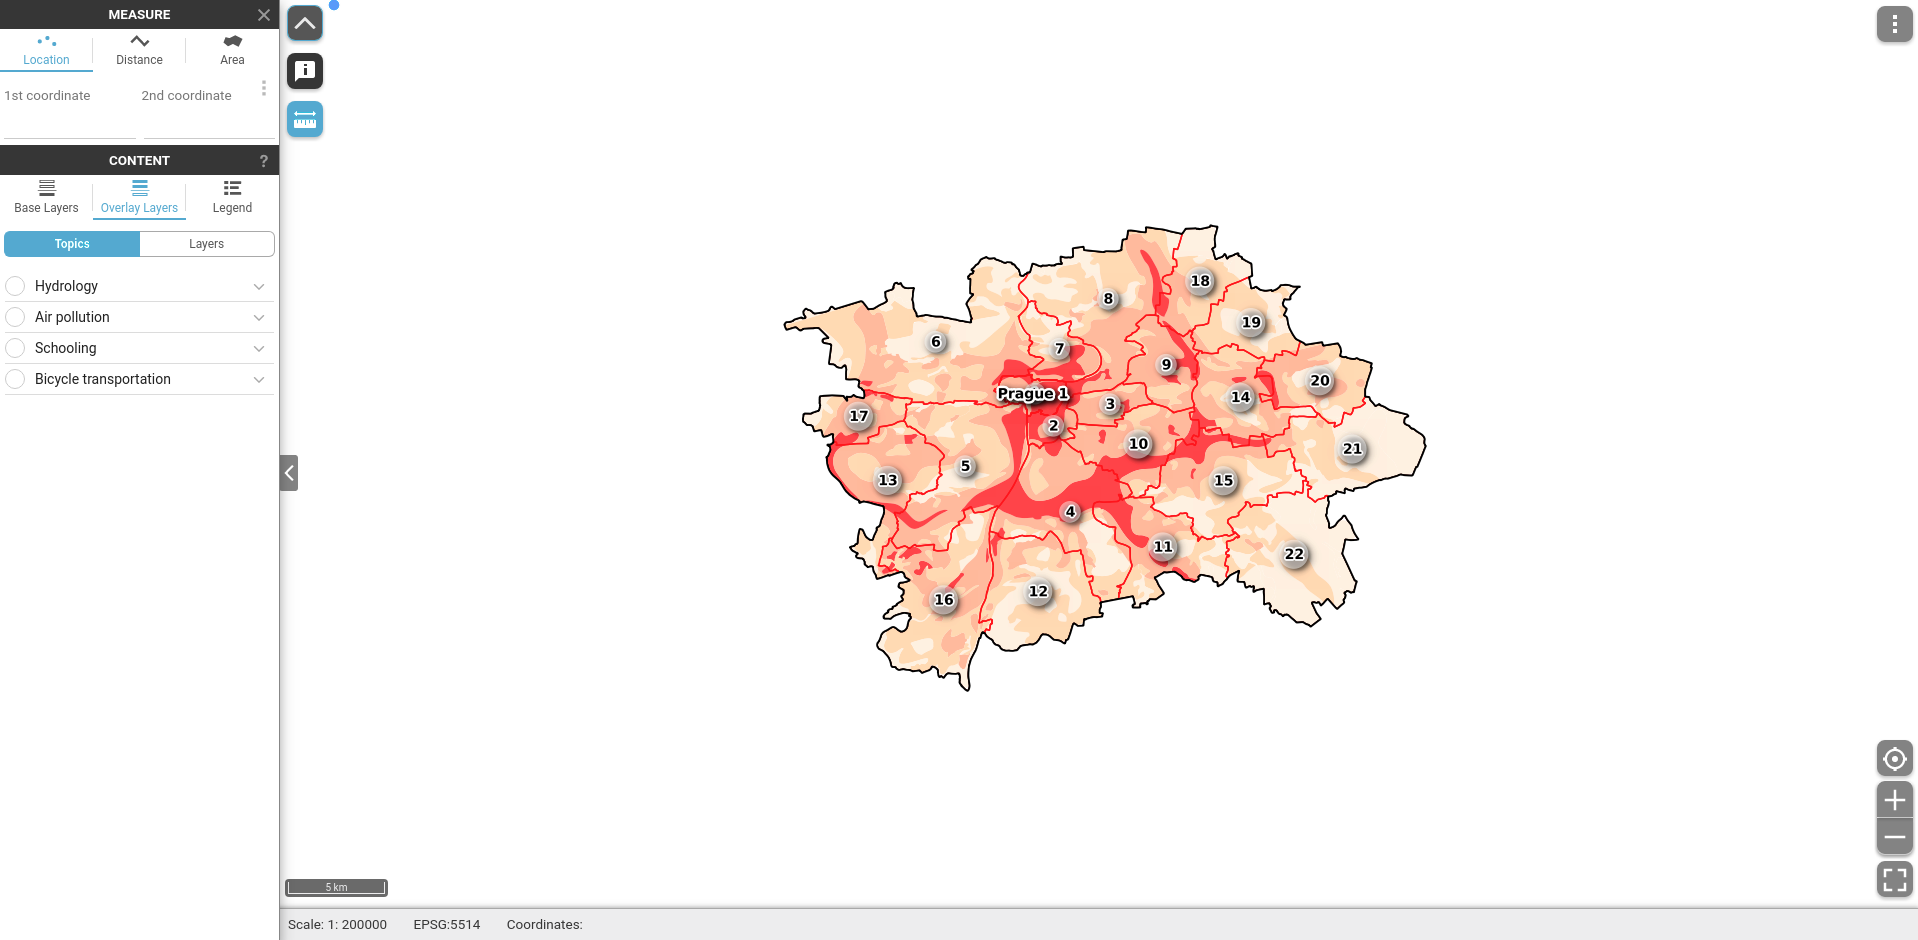
\includegraphics[width=0.9\textwidth]{../img/gisquick_ui.png}
	\caption{screenshot uživatelské rozhraní platformy Gisquick\cite{gisquick-prague}}
	\label{fig:gisquick-prague}
\end{figure}

Obrázek výše zachycuje webové uživatelské rozhraní Gisquick platformy. Jedná se o sadu velice jednoduchých a intuitivních nástrojů sloužících pro snadnou orientaci v publikovaném projektu, filtraci jednotlivých částí a provádění velice jednoduchých operací jako je například měření vzdáleností na mapě.

Uživatel má být schopný rychlé a intuitivní orientace v datech a samotné aplikaci. K tomu slouží postranní menu se správou vrstev spolu s menu nástrojů, které je v přiloženém obrázku rozbaleno. V postranním menu v horní části je právě aktivovaný nástroj sloužící k zjišťování souřadnic, měření vzdáleností a ploch. Hlavní část je věnována samotné interaktivní mapě. Ta poskytuje možnost změny velikosti a polohy zobrazovaného území.

\begin{figure}[h!]
	\centering
	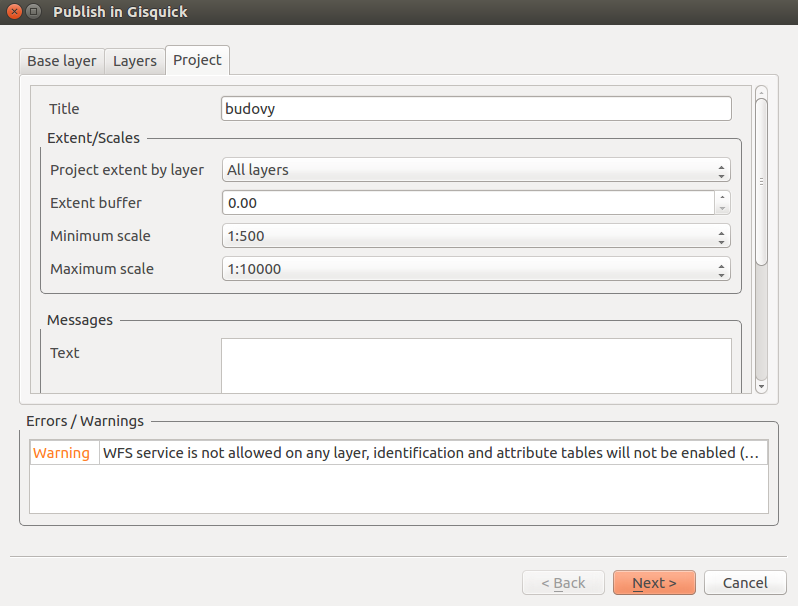
\includegraphics[width=0.7\textwidth]{../img/gisquick_plugin.png}
	\caption{screenshot uživatelské rozhraní Gisquick pluginu pro QGIS}
	\label{fig:gisquick-plugin}
\end{figure}

\newpage
Gisquick plugin rovněž disponuje uživatelským rozhraním, kde pomocí jednoduchého dialogového okna jsou nabízeny možnosti pro export vrstev. Jeho první část je rozdělena na tři záložky a stavovou řádku, kde se jsou vypisovány errory. V první záložce je možno nastavit podkladové vrstvy jako například Open Street Map, nebo Binq mapy. V další záložce je možno nastavit viditelnost jednotlivých vrstev. Při implementaci podpory pro časoprostorová data byly jednotlivé vrstvy rozšířeny o další nastavení. Tomu se bude práce věnovat detailněji v další části. V poslední záložce je obecné nastavení projektu. Další okno slouží k nastavení \textit{topics} nebo-li tématicky orientovaných vrstev \cite{gisquick-manual}. Předposlední stránka obsahuje pouze souhrn publikovaného projektu. A poslední zobrazuje výpis souborů, které se po zmáčknutí tlačítka \textit{Publish} vytvoří. Ty je poté nutné nahrát na Gisquick publikační server.

\newpage
\subsection{Použité technologie}
	
\begin{figure}[h!]
	\centering
	
\includegraphics[width=0.8\textwidth]{../img/technologies.JPG}
	\caption{loga níže popsaných softwarů}
	\label{fig:arcgis-time-settings}
\end{figure}	
	
\textbf{Vue.js} - jedná se o moderní framework s otevřeným kódem napsaný v programovacím jazyce JavaScript jehož první verze byla vydaná začátkem roku 2014 Evanem You \cite{vue-history}. Jeho hlavní použití je vývoj uživatelského rozhraní aplikací, tedy na straně klienta. Uživatelské rozhraní je za pomoci Vue.js rozděleno na několik  komponent, kdy každá obsahuje vlastní javascriptové, html a css skripty. Jednotlivé komponenty dělají kód přehlednější a aplikace méně náročnější. Protože vždy jsou použity jenom ty komponenty, které koncový uživatel potřebuje. Mezi další výhody Vue.js patří mimo práce s komponenty jeho reaktivita, možnosti routingu a úpravu objektového modulu dokumentu (DOM).  

Původní verze webového klienta Gisquicku jsou psány za použití frameworku AngularJS. V současné chvíli je však celý klient vytvářen znovu za pomoci medernějšího Vue.js. Z toho důvodu bylo rozšíření platformy o podporu časoprostorových dat na straně klienta psáno ve stejném framevorku Vue.js. Pokud by se nástroj osvědčil pro jeho použití v produkční verzi, nebude nutné do budoucna kód přepisovat.

\newpage
\bigskip
\noindent
\textbf{PyQt} - PyQt je vazba pro programovací jazyk Python, která umožňuje využití frameworku pro Qt aplikace. Vazby jsou vytvořeny ve formě Python modulů a obsahují okolo jednoho tisíce tříd. Jedná se o kombinaci výhod nabízející jednoduchost Pythonu a obrovské schopnosti Qt dohromady. Díky tomu je možné jednoduše vytvářet grafické uživatelské rozhraní přímo za pomocí Pythonu. PyQt je software s otevřeným kódem, který byl vytvořen britskou firmou Riverbank Computing a je nabízen pod dvojí licencí GNU GPL v3 a komerční licencí společnosti Riverbank \cite{pyqt}.

\bigskip
\noindent
\textbf{Docker} - Docker je počítačový program s otevřeným kódem umožňující zapouzdření (izolaci) jednotlivých aplikací do kontejnerů. Vytvořený kontejner se nazývá \textit{Docker image}. Obecné pravidlo je použití pouze jedné aplikace pro jeden Docker kontejner. Docker image mohou být posléze spuštěny na jakémkoli hardwaru s operačním systémem Linux, nebo Windows, na který je Docker program nainstalovaný. Tato skutečnost má obrovskou výhodu pro nasazení aplikací do produkčních serverů, jejich sdílení s dalšími uživateli, nebo vytváření clusterů složených z mikroservis. Po spuštění aplikace v Docker kontejneru není vytvořen nový virtuální stroj, ale aplikace v kontejnerech využívají hostující operační systém. Výhod tohoto řešení spočívá v minimalizaci velikosti kontejneru.

Gisquick pro deploy svých komponent (mimo Gisquick pluginu) v produkční verzi využívá právě použití Docker kontejnerů. Tímto způsobem je možné celou Gisquick platformu jednoduše spustit na lokálních zařízeních. Vývoj je tak jednodušší, protože odpadá jakékoli nastavování vývojového prostředí. 

\bigskip
\noindent
\textbf{Open Layers} - 

\newpage
\section{Implementace nástroje}

Následující kapitola popisuje způsob jakým byla platforma Gisquick respektive její komponenty rozšířeny o podporu práce s časoprostorovými daty. Jednotlivé podkapitoly zmiňují základní funkcionalitu, která byla nutná udělat a způsob její implementace.

\subsection{Gisquick plugin}
V kapitole 3.1 jsou zmíněny výstupy z Gisquick pluginu. Jedná se o sloužku obsahující projekt ve formátu .qgs, data použita v projektu a metadatový textový soubor. Soubor obsahuje nastavení a popis dat použité na straně mapového serveru a webového klienta. Hlavním cílem úprav Gisquick pluginu bylo tedy vytvoření jednoduchého uživatelského rozhraní, které umožní definovat všechny potřebná data, pomocí kterých budou do metadatového souboru vepsány potřebné informace identifikující vrstvu jako časovou. Ty poté souží ve webovém klientu k inicializaci nástroje pro práci s časovými daty.

\bigskip
\noindent
\textbf{Uživatelské rozhraní}

\begin{figure}[h!]
	\centering
	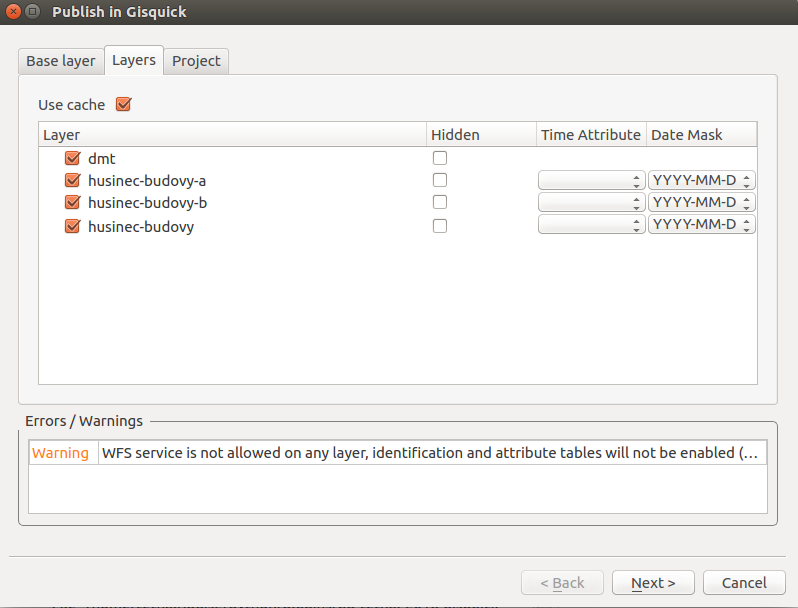
\includegraphics[width=0.9\textwidth]{../img/gisquick-plugin.png}
	\caption{nastavení vrstev v Gisquick pluginu}
	\label{fig:arcgis-time-settings}
\end{figure}

Obrázek 11 zobrazuje dialogové okno publikace projektu pomocí Gisquick pluginu. V prvním kroku publikace v záložce vrstvy \textit{Layers} je přidáno nové nastavení pro vektorové vrstvy. V Případě rastrových, jako je například v obrázku zvolená vrstva dmt, možnost nastavení časových vrstev není možná.

Ve sloupci \textit{Time Attribute} jsou v roletovém menu vypsány všechny atributy každé vrstvy. Implicitní nastavená hodnota je prázdný textový řetězec. Zde je nutné pro každou časovou vrstvu vybrat atribut, který obsahuje časové hodnoty. 

Sloupec \textit{Date Mask} obsahuje roletové menu s datovými masky, které určují jakým způsobem budou časová data na webovém klientu zobrazena. Díky tomuto nastavení je, nehledě na formát časového atributu, možné publikovat v časovém formátu, na který jsou cíloví uživatele zvyklí. V případě volby formátu je nutné znát původní data. Přejde se tím situacím kdy uživatel zvolí formát zobrazení dat pouze roky, zatímco původní data jsou v rozpětí jednoho dne.

Jestli jsou časové vrstvy dobře nastaveny se lze v předposledním kroku publikace přesvědčit v souhrnu publikovaného projektu.
%obrazek ze souhrnu (az bude)

\bigskip
\noindent
\textbf{Funkcionalita}

Poté co uživatel v záložce Vrstvy nastaví všechny požadované parametry může svou volbu potvrdit tlačítkem \textit{Next}, které spustí výpočet a zobrazí další krok publikace.

Do výpočetního procesu se dostanou pouze ty vrstvy, které splňují dvě podmínky. Jejich časový atribut \textit{Time Attribute} musí existovat. Tato podmínka eliminuje výpočet nad rastrovými vrstvy. Dále je nutné, aby byl nastavený časový atribut jiný než prázdný string. Tímto způsobem se do výpočtu dostanou pouze vrstvy, které uživatel výběrem atributu označí jako časové.

Výpočet probíhá pro jednotlivé vrstvy splňující vstupní podmínky totožně. Proces bude tety popsán pouze pro jednu.

V prvním kroku je vytvořena validační maska. Jedná se o pole, které svou velikostí odpovídá počtu mapových prvků \textit{Features} ve vrstvě. Každý prvek validační masky může nabývat dvou hodnot. Buďto obsahuje formát časového textového řetězce \textit{time string}, ve kterém je časová hodnota uložena. Pokud však časová hodnota není v textovém řetězci, nebo její časový formát textového řetězce neodpovídá podporovaným formátům, je do daného prvku validační masky uložena hodnota \textit{-1}. Podporované formáty jsou explicitně vypsány ve zdrojovém kódu Gisquick pluginu.

Pro vrstvu obsahující šest prvků, kdy pouze pět z nich má validní datum a to ještě v odlišných časových formátech může validační maska vypadat následovně:

\begin{verbatim}
[
  '%Y-%m-%d',
  '%Y-%m-%d',
  -1,
  '%Y-%m-%dT%H:%M:%S',
  '%Y-%m-%dT%H:%M:%S',
  '%Y-%m-%dT%H:%M:%S'
]
\end{verbatim}

Během vytváření validační masky jsou rovnou data kontrolována. Díky tomu je možné zjistit jak maska vypadá aniž by bylo nutné její jednotlivé prvky procházet. Po její vytvoření jsou pouze tři možné scénáře jsou možné.

\begin{itemize}
	\item\textit{Data nejsou validní} - znamená, že ani jeden hodnota v zadaném časovém atributu nemá validní časovou hodnotu. Validační maska tedy obsahuje pouze hodnoty \textit{-1}. Výpočet je v tomto případě ukončen.
	\item\textit{Data jsou validní a obsahují pouze jeden časový formát} - v tomto případě je zjištěno, jestli je časový formát neobsahuje speciální znak, který by jeho použití v původní podobě znemožnil.
	\begin{itemize}
		\item\textit{Obsahuje speciální znak} - v tom případě se pokračuje způsobem stejným jako v případě \item\textit{Data jsou validní, ale obsahují více časových formátů}
		\item\textit{neobsahuje speciální znak} - časové textové řetězce jsou za pomocí zjištěného časového formátu převedeny do časového formátu \textit{UNIX TIME}. Z těchto hodnot jsou poté zjištěny jejich maximální a minimální hodnota.
	\end{itemize}
	\item\textit{Data jsou validní, ale obsahují více časových formátů} - jedná se tedy o validní nekonzistentní data. K tomu aby vrstvu s těmito časovými hodnoty bylo možné označit za časovou je nutné vytvořit nový atribut, který obsahuje časové hodnoty v jednotném formátu. Toho je docíleno pomoci validační masky, kdy se prochází jednotlivé hodnoty a pokud pro ně existuje formát časového textového řetězce, jsou převedeny do formátu \textit{UNIX TIME}. Ten je následně uložen v novém atributovém sloupci. V případě nevalidní časové hodnoty je pole prázdné. Na základě hodnot v atributu obsahující časové hodnoty ve formátu \textit{UNIX TIME} je určena hodnota minimálního a maximálního časového atributu.
	V případě, že nový atribut již jednou vytvořen byl, jsou jeho hodnoty přepsány.
\end{itemize}

Posledním krokem je poté pouze export zjištěných hodnot do metadatového souboru. Pro každou časovou vrstvu je vypsána časový formát pro zobrazení hodnot na webovém klientu. Dále název časového atributu, minimální a maximální hodnota časového atributu ve formátu \textit{UNIX TIME} a další parametry které budou popsány a vysvětleny dále. V případě, že data jsou validní a není vytvořen nový atribut obsahující časové hodnoty ve formátu \textit{UNIX TIME} je vypsán formát obsažený ve validační masce. Pokud je atribut vytvořen je vypsán jeho název.

%vyvojovy diagram

\bigskip
\noindent
\textbf{Metadatový soubor}

Metadatový soubor je textový soubor, který vniká publikací projektu pluginem Gisquick. Obsahuje množství informací, které jsou nutné pro správnou konfiguraci straně mapového serveru a webového klienta. V případě časových vrstev jsou dodatečné informace použité pouze na straně webového klienta. 

Pokud jsou vrstvy při publikaci označeny jako časové a jejich data jdou validní, jsou do nich vepsány následující hodnoty:

\begin{itemize}
	\item\textit{unix} - parametr unix nabývá hodnoty \textit{TRUE} v případě, že byl vytvořen nový atribut s časovými hodnoty ve formátu \textit{UNIX TIME}. Slouží webovému klientu k určení zdali k filtrování časové vrstvy má použít daný formát, nebo \textit{UNIX TIME}.
	\item\textit{originalTimeAttribute} - zde je uložen název časového atributu. Parametr slouží k určení atributu při filtrování časové vrstvy. 
	\item\textit{outputDatetimeMask} - obsahuje formát časového řetězce, který si uživatel zvolil v roletovém menu \textit{Date Mask}. Použití tohoto parametru je pouze pro možnost definice formátu zobrazení data a času v časovém nástroji.
	\item\textit{timeValues} - jedná se o pole obsahující minimální a maximální hodnotu časového atributu ve formátu \textit{UNIX TIME}. Dle těchto hodnot je inicializovaný časový posuvník. 
	\item\textit{inputDatetimeMask} - tento parametr je vytvořen pouze pokud není nutné vytvářet nový atribut obsahující hodnoty ve formátu \textit{UNIX TIME}. Parametr obsahuje formát časového řetězce pro zvoleného časového atributu. Díky tomuto parametru může být pro potřeby filtrování časové vrstvy převedena hodnota učená na časovému posuvníku do stejného časového formátu v jakém je uložena. 
	\item\textit{timeAttribute} - parametr je vytvořen pouze pokud je nutné vytvářet nový atribut obsahující hodnoty ve formátu \textit{UNIX TIME}. Obsahuje název nově vytvořeného atributu. Parametr slouží stejně jako \textit{originalTimeAttribute} k určení atributu při filtrování časové vrstvy.  
\end{itemize}



\newpage
\subsection{Webový klient}

Jejich výčtem je možné obecně určit nutné data, která jsou pro práci s časoprostorovými nezbytná:

\begin{itemize}
	\item \textit{časové hodnoty} - jedná se o nejdůležitější data, na kterých je závislé nastavení dílčích nástrojů pro časovou filtraci a vytváření animace na základě časové osy. Jedná se o interval hodnot, definovaný minimální a maximální
\end{itemize}

%\section{Gisquick plugin pro QGIS}

%\subsection{Mapy a internet}

